\documentclass[12pt, a4paper]{article}
\usepackage[UKenglish]{babel}
\usepackage[utf8]{inputenc}
\usepackage{mathtools} % an extension of amsmath
\usepackage{amsthm, amssymb, amsfonts, amstext}
\usepackage{longtable}
\usepackage{tocloft}
\usepackage{geometry}
\usepackage{algpseudocode}
\usepackage{multicol}
% \geometry{margin=10mm, bottom=18mm, top=18mm}
\geometry{margin=24mm}
\usepackage{listings}
\usepackage[x11names]{xcolor} % for a list of colours: https://mirror.mwt.me/ctan/macros/latex/contrib/xcolor/xcolor.pdf#page=40&zoom=auto,-214,513
\usepackage{colortbl}
\usepackage{wrapfig}
\usepackage{graphicx}
\usepackage{array}
\usepackage{tabularx}
\usepackage{makecell}
\usepackage{ulem}
\usepackage{enumitem}
\usepackage[many]{tcolorbox} 
% \setlist{noitemsep} % remove space between items in list
% \setlist{nolistsep} % even more compact lists

% \def\darkmode{1}
\ifdefined \darkmode
\definecolor{pageBG}{rgb}{0.11,0.11,0.11}
\pagecolor[RGB]{35,35,35}
\color[rgb]{1,1,1}
\else
\definecolor{pageBG}{rgb}{1,1,1}
\fi
\newtcolorbox{mybox}[3][] {
    colframe = #2!25,
    colback  = #2!10,
    coltitle = #2!20!black,  
    title    = {#3},
    #1,
  }
% Usage:
%\begin{mybox}[breakable]{red}{Title}
%    contents
%\end{mybox}
\renewcommand\theadalign{bc} % to leave lines inside a table
\renewcommand\theadgape{\Gape[4pt]}
\renewcommand\cellgape{\Gape[4pt]}
\usepackage{hyperref}
\ifdefined \darkmode
\hypersetup{
    colorlinks=true,
    linkcolor=Aquamarine1,
    filecolor=magenta,
    urlcolor=cyan,
}
\else
\hypersetup{
    colorlinks=true,
    linkcolor=blue,
    filecolor=magenta,
    urlcolor=cyan,
}
\fi
\ifdefined \darkmode
\lstdefinestyle{mystyle}{
    backgroundcolor=\color{pageBG},
    commentstyle=\color{Chocolate1},
    keywordstyle=\color{PaleTurquoise1},
    numberstyle=\color{Magenta1},
    stringstyle=\color{CadetBlue1},
    basicstyle=\ttfamily\footnotesize\color{white},
    breakatwhitespace=false,
    breaklines=true,
    captionpos=b,
    keepspaces=true,
    numbers=left,
    numbersep=5pt,
    showspaces=false,
    showstringspaces=false,
    showtabs=false,
    tabsize=4
}
\else
\lstdefinestyle{mystyle}{
    backgroundcolor=\color{white},
    commentstyle=\color{SlateGray4},
    keywordstyle=\color{SeaGreen4},
    numberstyle=\color{VioletRed4},
    stringstyle=\color{Blue4},
    basicstyle=\ttfamily\footnotesize\color{black},
    breakatwhitespace=false,
    breaklines=true,
    captionpos=b,
    keepspaces=true,
    numbers=left,
    numbersep=5pt,
    showspaces=false,
    showstringspaces=false,
    showtabs=false,
    tabsize=4
}
\fi
\lstset{style=mystyle}
\urlstyle{same}
\usepackage{cleveref}
\usepackage{bm}
\newcommand{\bs}{\boldsymbol}
\usepackage{titling}
\setlength{\droptitle}{-5em} % to move the title up/down
\usepackage{etoolbox}

\newtheorem{theorem}{Theorem}[section]
\theoremstyle{definition}
\newtheorem{definition}{Definition}[section]
\newtheorem*{claim}{Claim}
\theoremstyle{remark}
\newtheorem*{remark}{Remark}
% \numberwithin{equation}{section}
\newcommand{\textsb}{\textsubscript}

\usepackage{placeins}
\pretocmd{\section}{\FloatBarrier}{}{}
%\pretocmd{\subsection}{\FloatBarrier}{}{}
%\pretocmd{\subsubsection}{\FloatBarrier}{}{}

% Set width in tables column-wise while allowing for automatic line breaks
% left fixed width:
\newcolumntype{L}[1]{>{\raggedright\arraybackslash}p{#1}}
% center fixed width:
\newcolumntype{C}[1]{>{\centering\arraybackslash}p{#1}}
% flush right fixed width:
\newcolumntype{R}[1]{>{\raggedleft\arraybackslash}p{#1}}
% example:
% \begin{table}[!htbp]
%   \centering
%     \begin{tabular}{L{1cm}L{9cm}}
% ...
\usepackage[export]{adjustbox}

\newenvironment{QandA}{\begin{enumerate}[label=\bfseries\arabic*.]\bfseries}
    {\end{enumerate}}
\newenvironment{answered}{\par\normalfont}{}

\title{Embedded Systems Workshop Project\\PID Control of DC Motor}
\author{\uline{Team 35}\\Aditya Harikrish - 2020111009\\Lokesh Venkatachalam - 2020111017\\Nitin Rajasekar - 2020101117\\Saurav Chhatani - 2020101113}
\date{}

\begin{document}
\maketitle
\tableofcontents
\newpage

\section{Motivation}
Feedback controls loops are widely used in several industries in order to precisely control actuators to produce the desired output.
A seemingly easy problem at first glance, it shows its challenges with a deeper dive.
PID controllers find use in almost all major automated processes due to low maintenance cost and high reliability.
They are generally the go-to choice for applications which require constant maintenance of some fixed system parameter.
Some places where PID controllers find use are to maintain flow of liquids, regulate the temperature, monitor radiation levels, and maintain pressure in pressurised chambers.

\section{Block diagram/circuit diagram of the hardware}
\begin{figure}[!h]
    \centering
    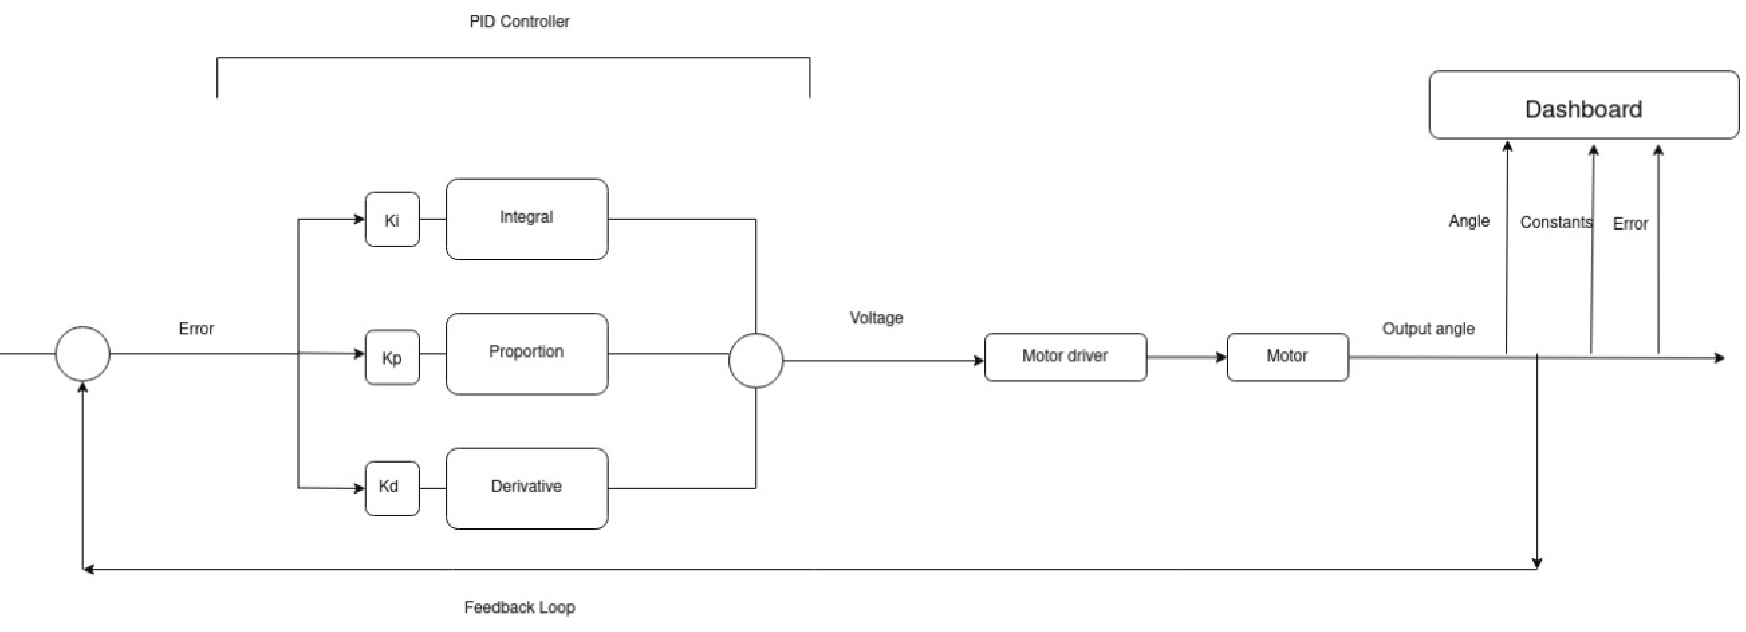
\includegraphics[scale=0.2]{img/block1.png}
    \caption{Workflow of the main circuitry}
    \label{fig:block1}
\end{figure}

\begin{figure}[!h]
    \centering
    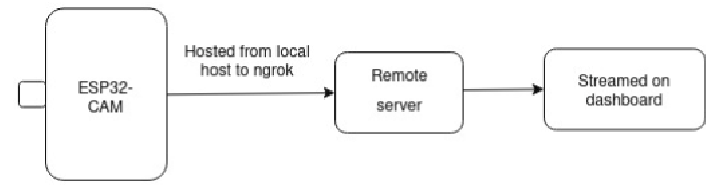
\includegraphics[scale=0.2]{img/block2.png}
    \caption{Workflow of the camera circuitry}
    \label{fig:block2}
\end{figure}

\section{Methodology}
A proportional-integral-derivative (PID) controller is a control loop mechanism used to ensure that the output of an actuator reaches a desired value by iteratively updating the input given to the actuator. In our case, the sensor attached to the motor measures the angle by which it has turned and the actuator is the motor itself. The setpoint and program variable are the angles turned by the motor and the input given to the motor is power.

The desired value is called the setpoint ($SP$) and the current output of the actuator is called the program variable ($PV$). The error term, $e(t)$ is defined as the difference between $SP$ and $PV$ at the $i$th timestep. The input to be given to the actuator at the $i$th timestep is calculated as
\begin{equation}\label{eq:PID}
    u(t) = K_p e(t) + K_i \int_{0}^{t} e(x) dx + K_d \frac{de(t)}{dt}.
\end{equation}

\subsection{P Controller}
\begin{equation}
    u(t) = K_p e(t)
\end{equation}
The proportional component is directly proportional to the error and is large when $PV$ is far from $SP$. Without the integral and derivative components, $u(t)$ would become 0 when $e(t) = 0$. In the case of infinitesimally small resolutions of both, the protractor and the encoder, this alone would suffice for controlling the angle of the motor.

However, consider the example of a drone that starts from the ground level and needs to be elevated 50m. Suppose the input to the drone is the angular velocity of the fans of the drone. At the height of 50 m, $e(t) = 0 \Rightarrow K_p e(t) = 0$ and it is similarly small when $e(t)$ is small. The drone would thus never reach the setpoint of 50 m and instead hover at some height $h < 50$ m where $K_p e(t)$ balances the weight of the drone. This is called the steady state error.

\subsection{PI Controller}
\begin{equation}
    u(t) = K_p e(t) + K_i \int_{0}^{t} e(x) dx
\end{equation}
The integral component is added to bring the steady state error to 0 by accounting for the past errors. At the steady state, $e(t)$ is nonzero and thus integrating it also produces a nonzero term.

However, this causes oscillations around the setpoint due to the constant overshooting and undershooting of the setpoint. This is called the integral windup.

\subsection{PID Controller}
While the PI controller does reach the destination, the path it takes to do so need not be optimal due to the oscillations. The derivative component in \ref{eq:PID} is added to predict the future respond to how fast the drone is closing in on the setpoint.

While just the P controller would suffice in the case of getting a motor to rotate by some angle (since there is no force to cause a steady state error), we have implemented a PID controller as a proof of concept for the use of PID controllers in more complex systems.

\section{Deployment campaign}
The oneM2M server is hosted remotely, to allow for free access to its data from the microcontroller, without having the connect both of them to the same network.

\section{Data validation}
The final program variables measured using the attached protractor when various setpoint angles are inputted through the dashboard are shown in \cref{fig:calibration}. The absolute error is measured to be at most $2^\circ$. This is due to the fact that the optical encoder attached to the motor measures a full circle in 420 steps, which implies that its resolution is $360/420 ^\circ \approx 0.86 ^\circ$. However, the protractor's resolution is $1^\circ$. Due to the mismatch, the error is at most $2^\circ$.

\begin{figure}[!h]
    \centering
    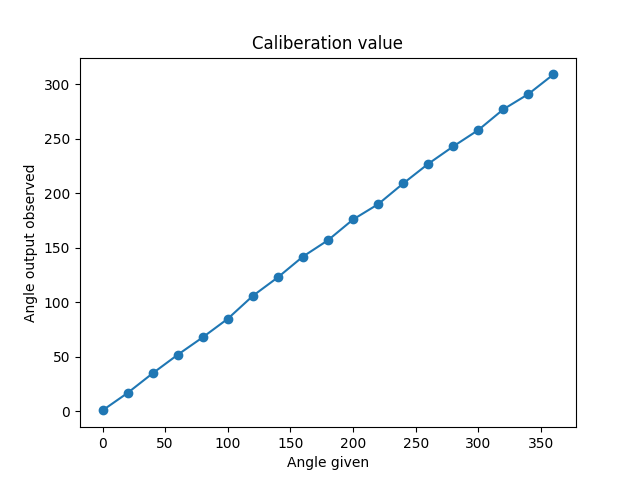
\includegraphics[scale=0.8]{img/calibration.png}
    \caption{Home page when logged out}
    \label{fig:calibration}
\end{figure}

\section{Flow diagram/chart of the entire data flow pipeline}
The user's credentials are stored in the MongoDB Atlas server. After the user logs in, data from the ThingSpeak channel is fetched and displayed on the dashboard. The user can then input the setpoint angle and the ESP32 attached to the DC motor will make the latter rotate by that angle. Then, it pushes the updated data of the setpoint, program variable, error, $K_p$, $K_i$, and $K_d$ to ThingSpeak in a single push. The dashboard then fetches the data from ThingSpeak and displays it on the dashboard.

The other data flow loop is for the camera feed, which the ESP32-CAM sends to an ngrok server, which is then sent to the dashboard.

\begin{figure}[!h]
    \centering
    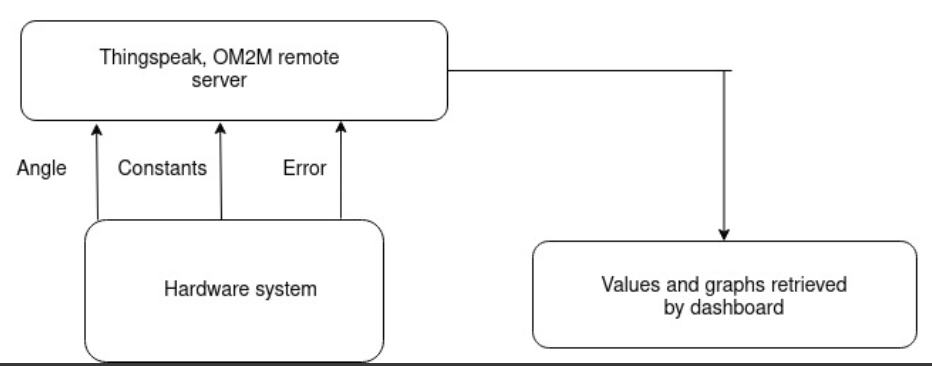
\includegraphics[scale=0.4]{img/dataflow.png}
    \caption{Home page when logged out}
    \label{fig:dataflow}
\end{figure}

\section{Communication to ThingSpeak and oneM2M}
The microcontroller (ESP32-CAM) reads the angle turned by the motor and sends it to field1 of the ThingSpeak channel. The ThingSpeak channel is then used to send the data to the oneM2M server. The oneM2M server is then used to send the data to the dashboard.

\section{Development of dashboard}
The dashboard has been developed using the MERN stack (MongoDB, ExpressJS, ReactJS, and NodeJS). The frontend is responsive, and interacts with the database in ThingSpeak. The user database is hosted on MongoDB Atlas. The dashboard is hosted remotely. The backend is robust, portable, and secure.

\begin{figure}[!h]
    \centering
    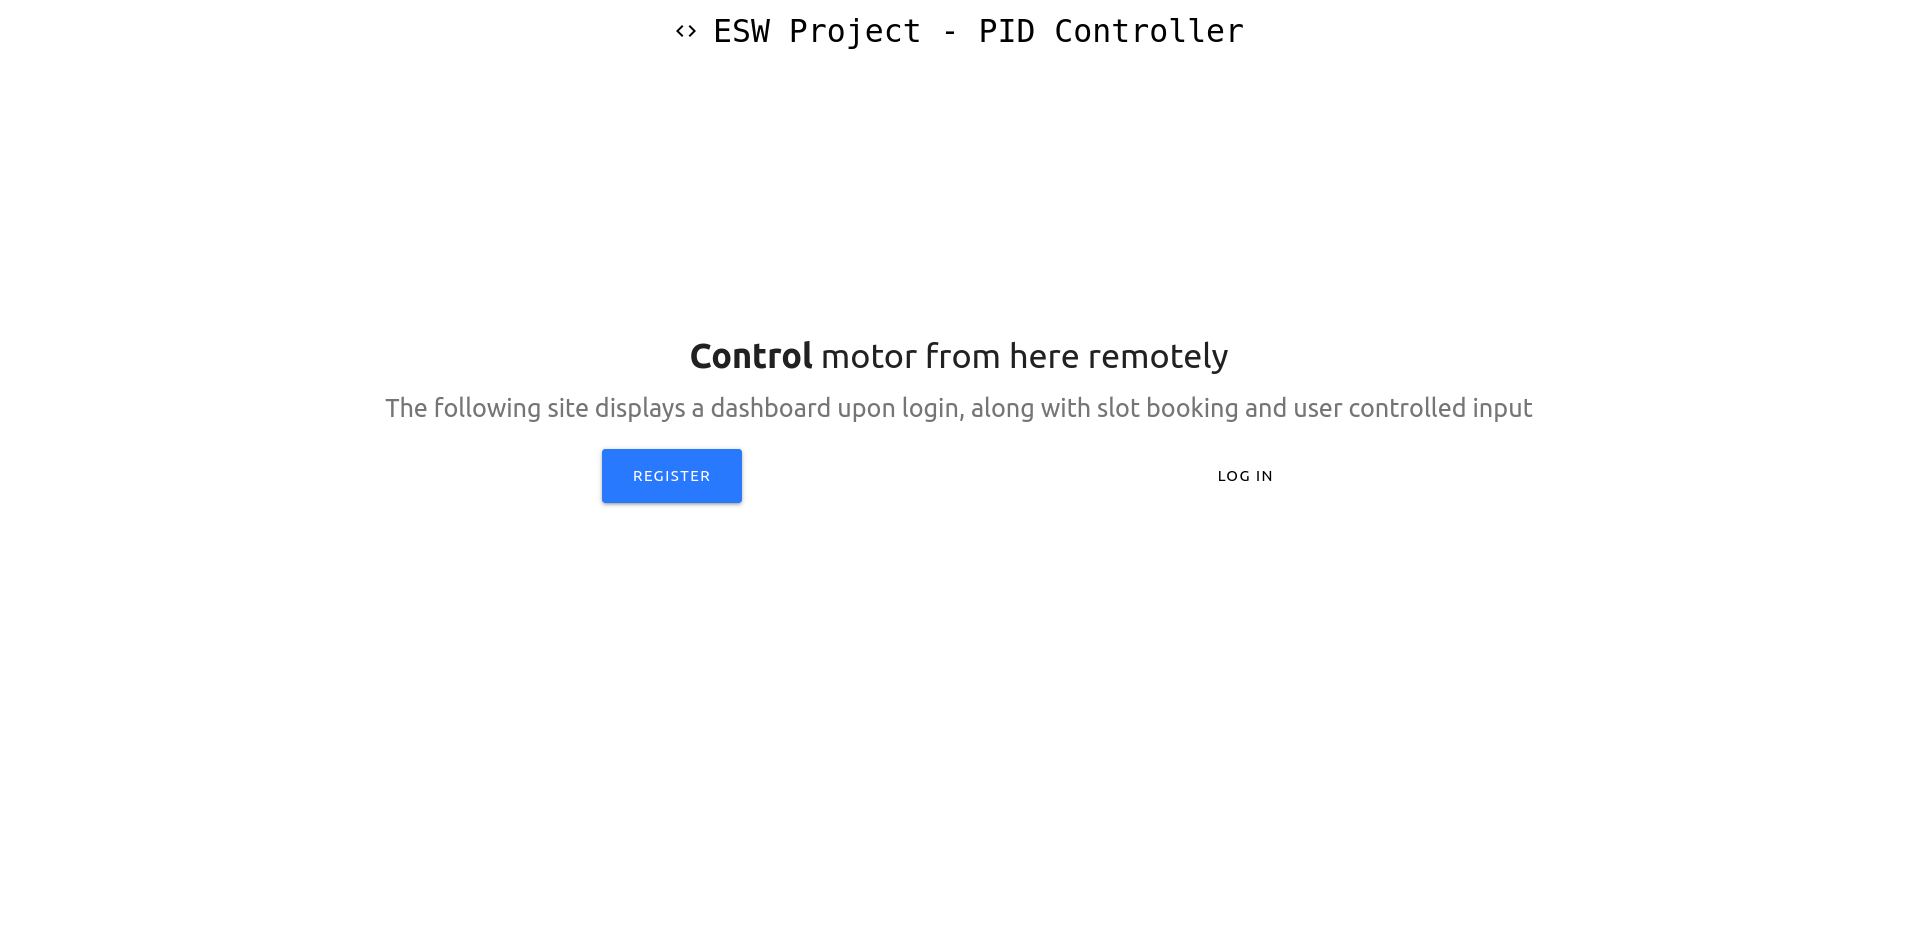
\includegraphics[scale=0.2, frame]{img/1.png}
    \caption{Home page when logged out}
    \label{fig:1}
\end{figure}

\begin{figure}[!h]
    \centering
    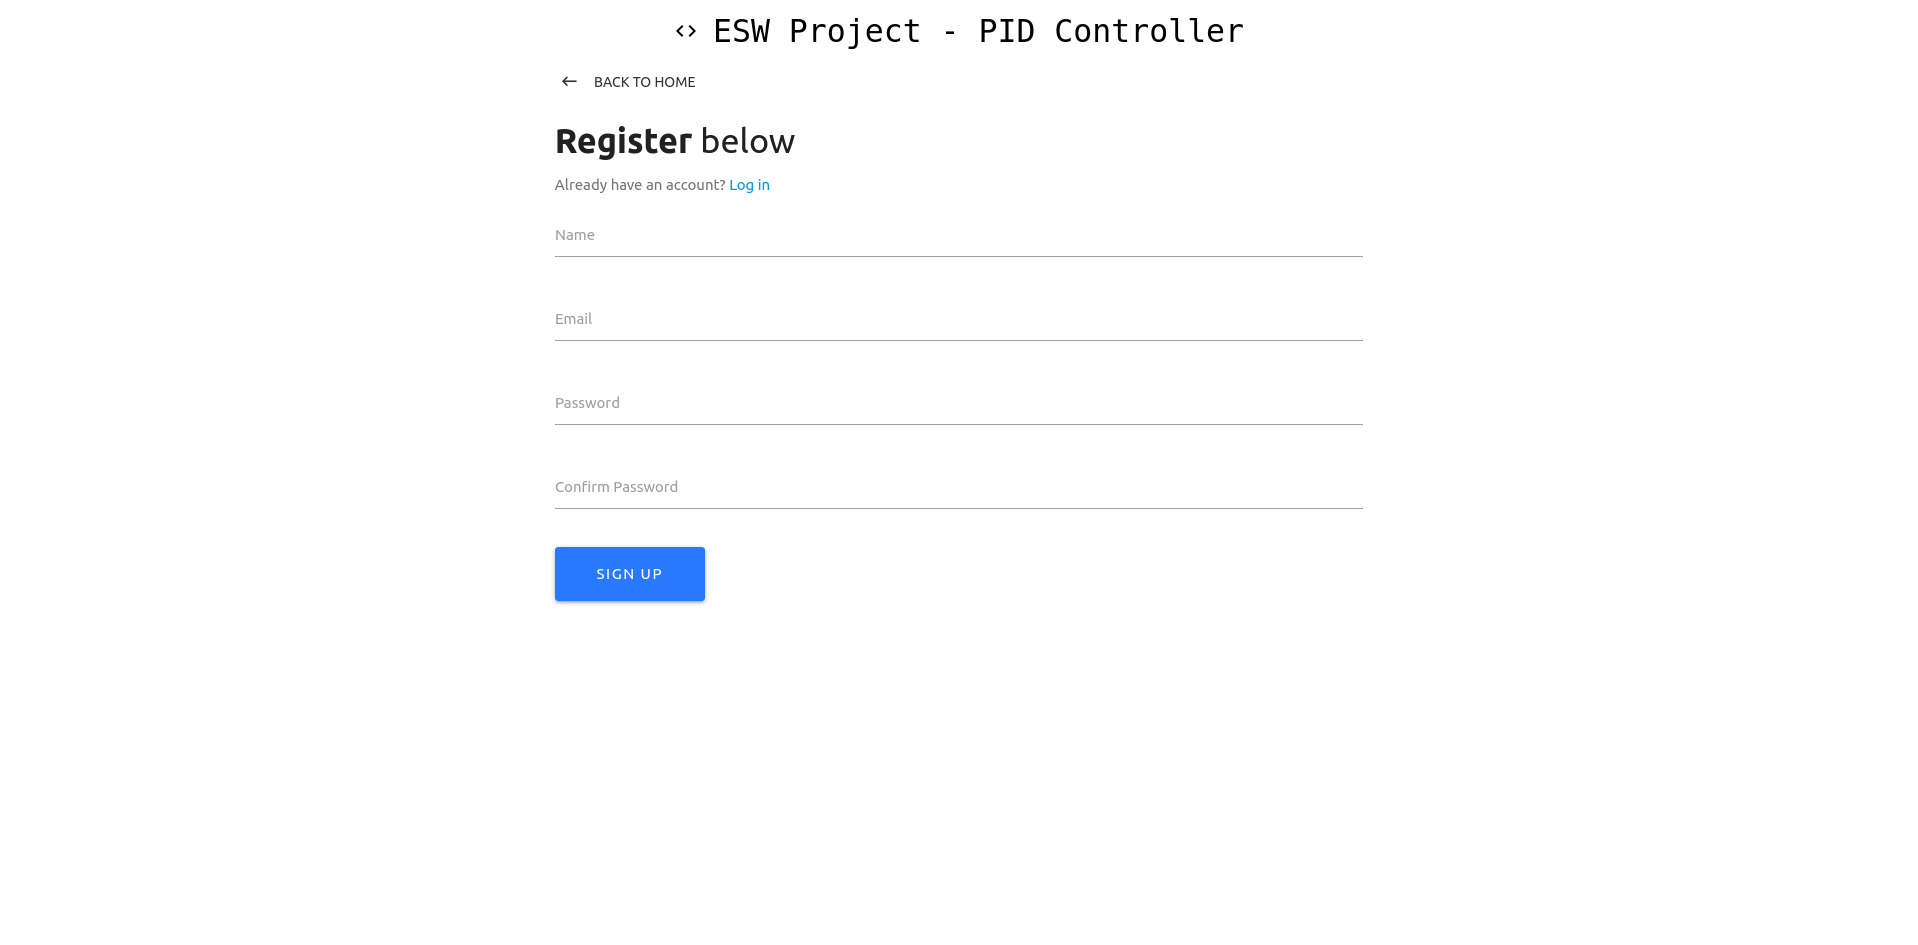
\includegraphics[scale=0.2]{img/2.png}
    \caption{Registration Page}
    \label{fig:2}
\end{figure}

\begin{figure}[!h]
    \centering
    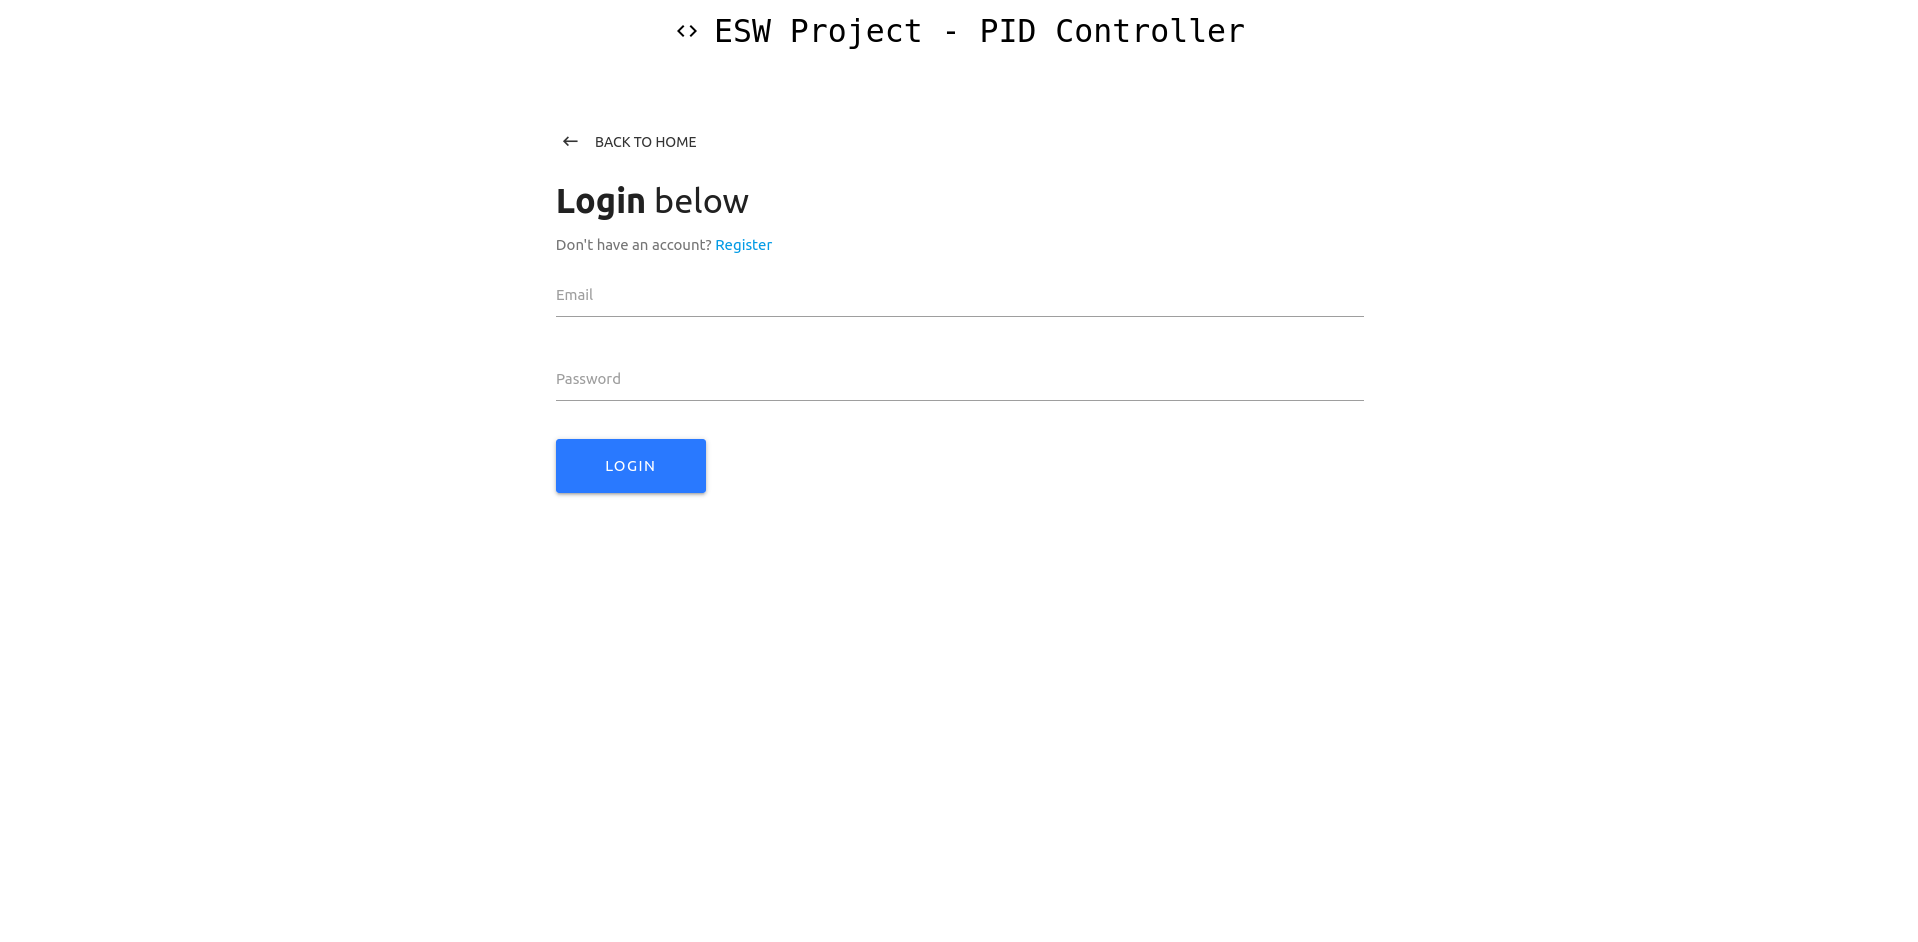
\includegraphics[scale=0.2]{img/login.png}
    \caption{Login page}
    \label{fig:3}
\end{figure}

\begin{figure}[!h]
    \centering
    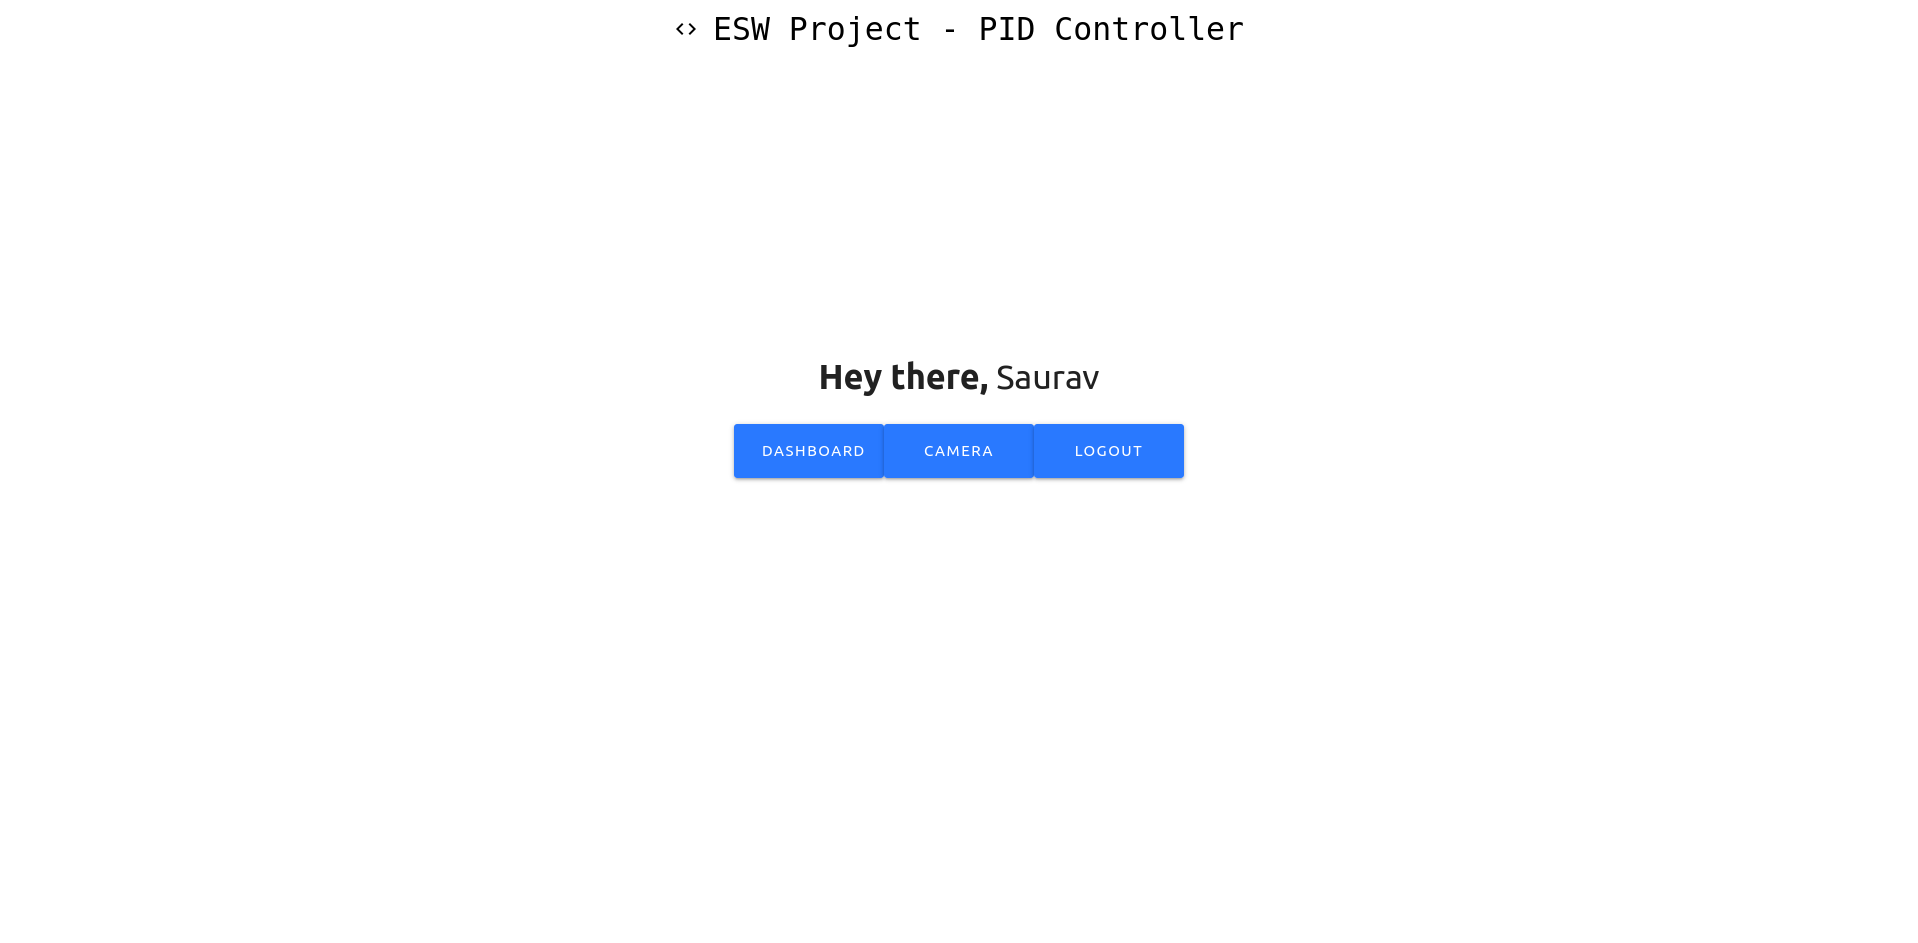
\includegraphics[scale=0.2]{img/loggedin_homepage.png}
    \caption{Login page}
    \label{fig:4}
\end{figure}

\begin{figure}[!h]
    \centering
    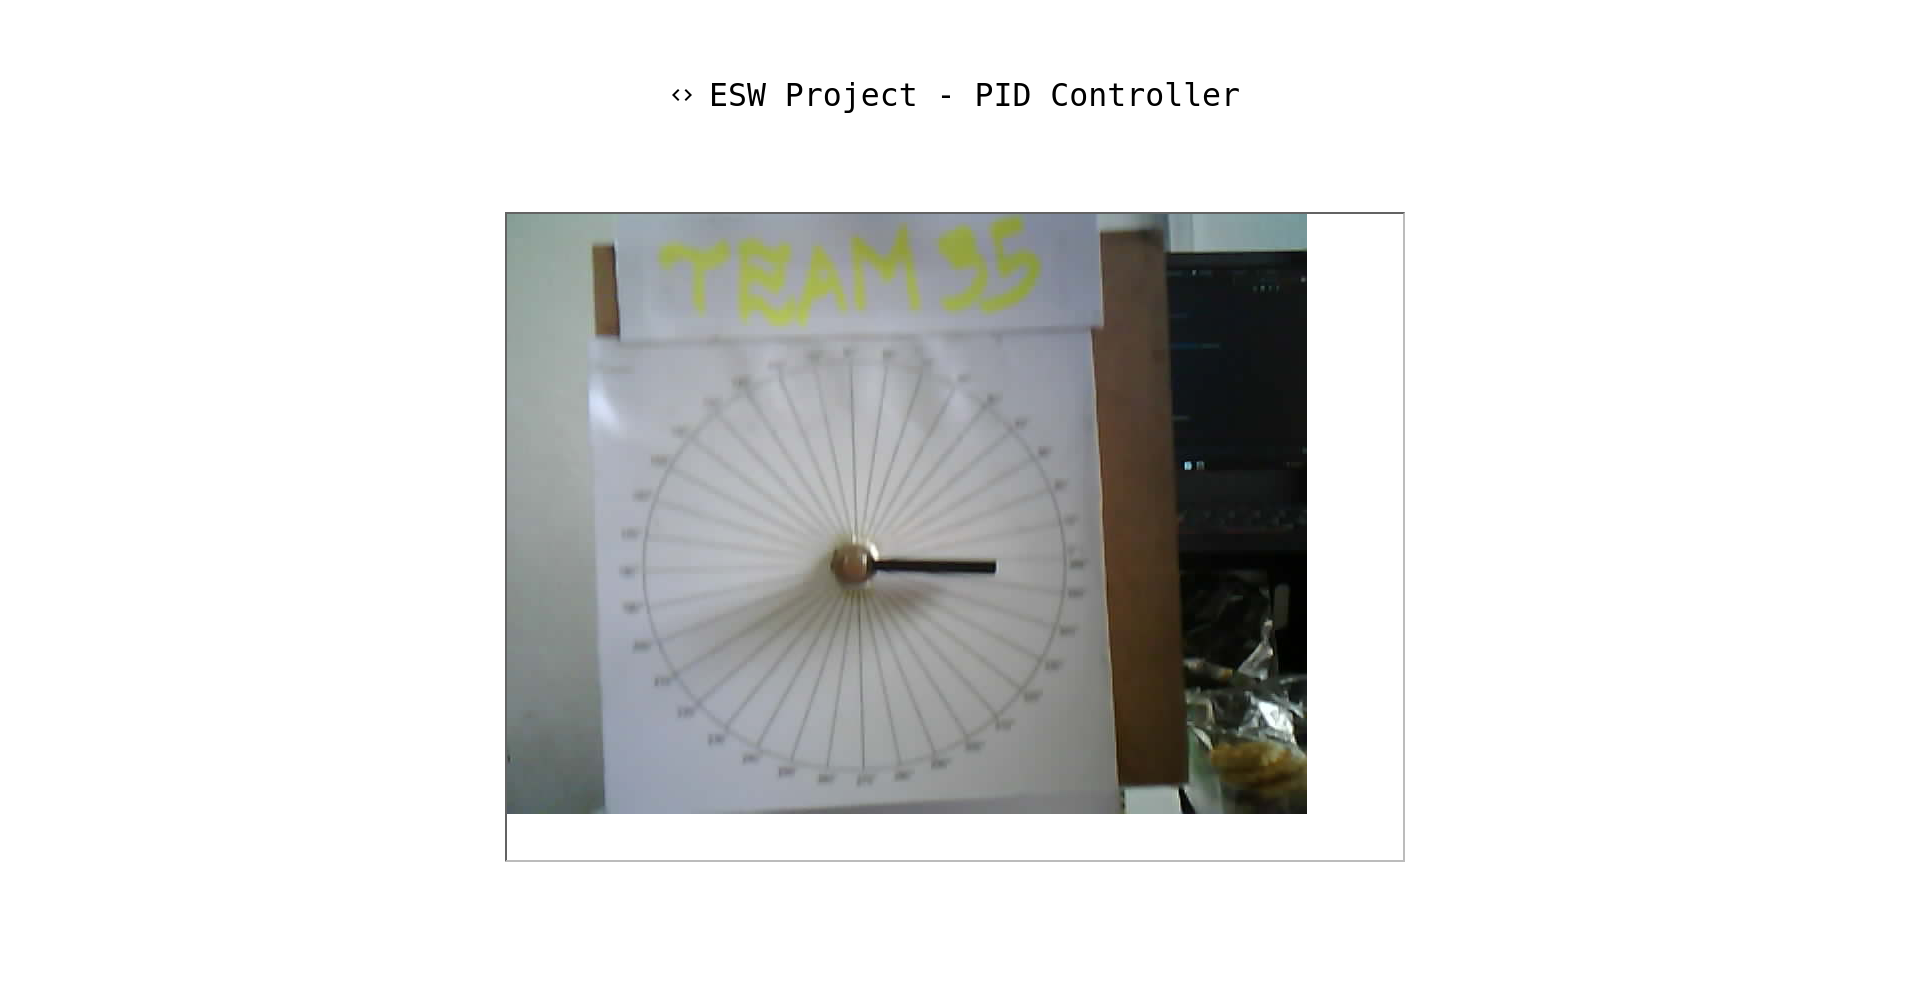
\includegraphics[scale=0.2]{img/video_feed.png}
    \caption{Live camera feed in the dashboard}
    \label{fig:6}
\end{figure}

\section{Use of IoT security tools in your project}
The microcontroller is connected to the internet via a WiFi network. The WiFi network is secured using WPA2-PSK. The microcontroller and the dashboard are connected to the ThingSpeak channel using private read and write API keys.

\section{Data visualization and analysis}
Through a large number of trial-and-error experiments, we arrived at a ratio for the combination of values for $K_p$, $K_i$, and $K_d$ that minimises the error and lets the motor reach the setpoint in the fastest possible time. We landed upon the ratios $K_p / K_d = 100$, while $K_p / K_d = 2$.

This experimental analysis is reflected in the dashboard, where the default values are in this ratio (see \cref{fig:5}).

\begin{figure}[!h]
    \centering
    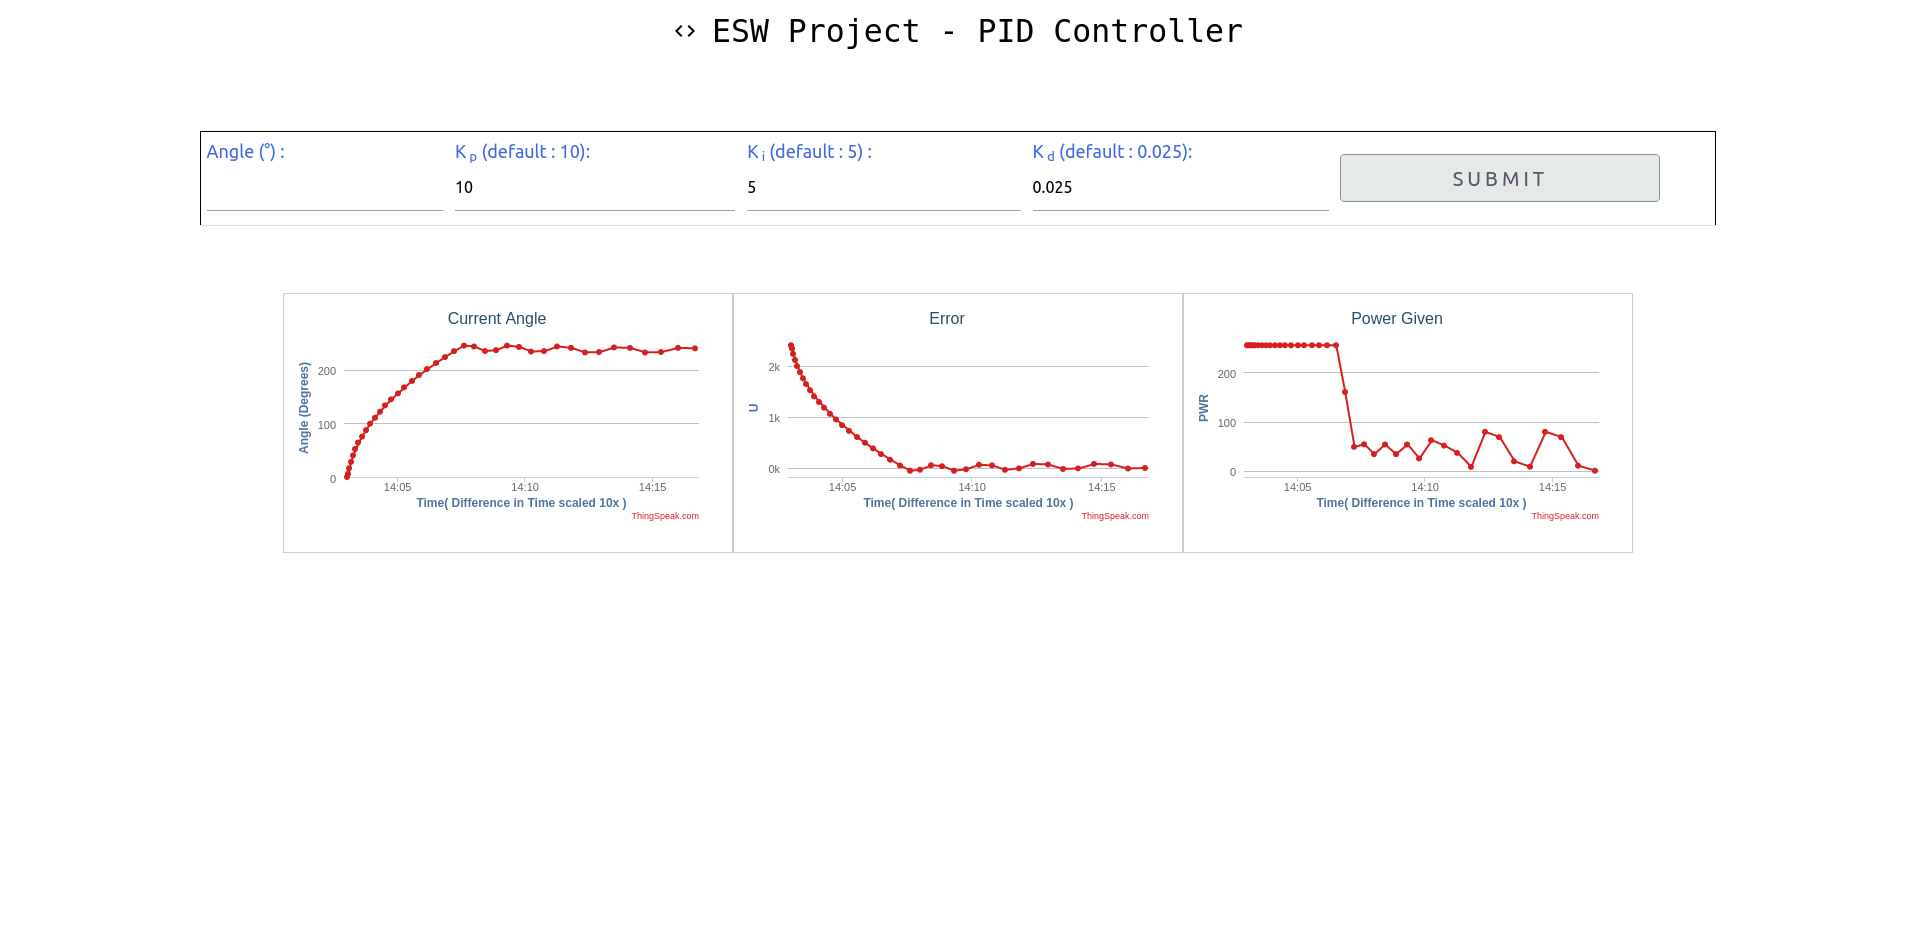
\includegraphics[scale=0.2]{img/dashboard.png}
    \caption{Data visualisation in the dashboard}
    \label{fig:5}
\end{figure}

\section{Final results and conclusion }
Users can remotely register, log in, and get the motor to turn by a desired angle during their booked slots. The dashboard also allows users to view the live camera feed from the microcontroller, to change the PID controller parameters, and view live the data visualisation of the motor's angle.

\section{Final code base}
Please click \href{https://github.com/LokeshVenkatachalam/PID-Control-DC-motor}{here} to go to the GitHub repository.

\end{document}

